
\subsubsection{NoiseMiner View}

The NoiseMiner view (see figure \ref{time profile}) displays statistics about abnormally long entry methods. The abnormal events are filtered and clustered across multiple dimensions to produce a concise summary. The view displays both the duration of the events as well as the periodicity at which they occur. Its dialog box is exactly the same as that of the Graph tool (see section \ref{sec::graph view}).

The tool uses stream mining techniques to produce its results by making only one pass through the input data while using a limited amount of memory. This allows NoiseMiner to be very fast. 

\begin{figure}[htb]
\center
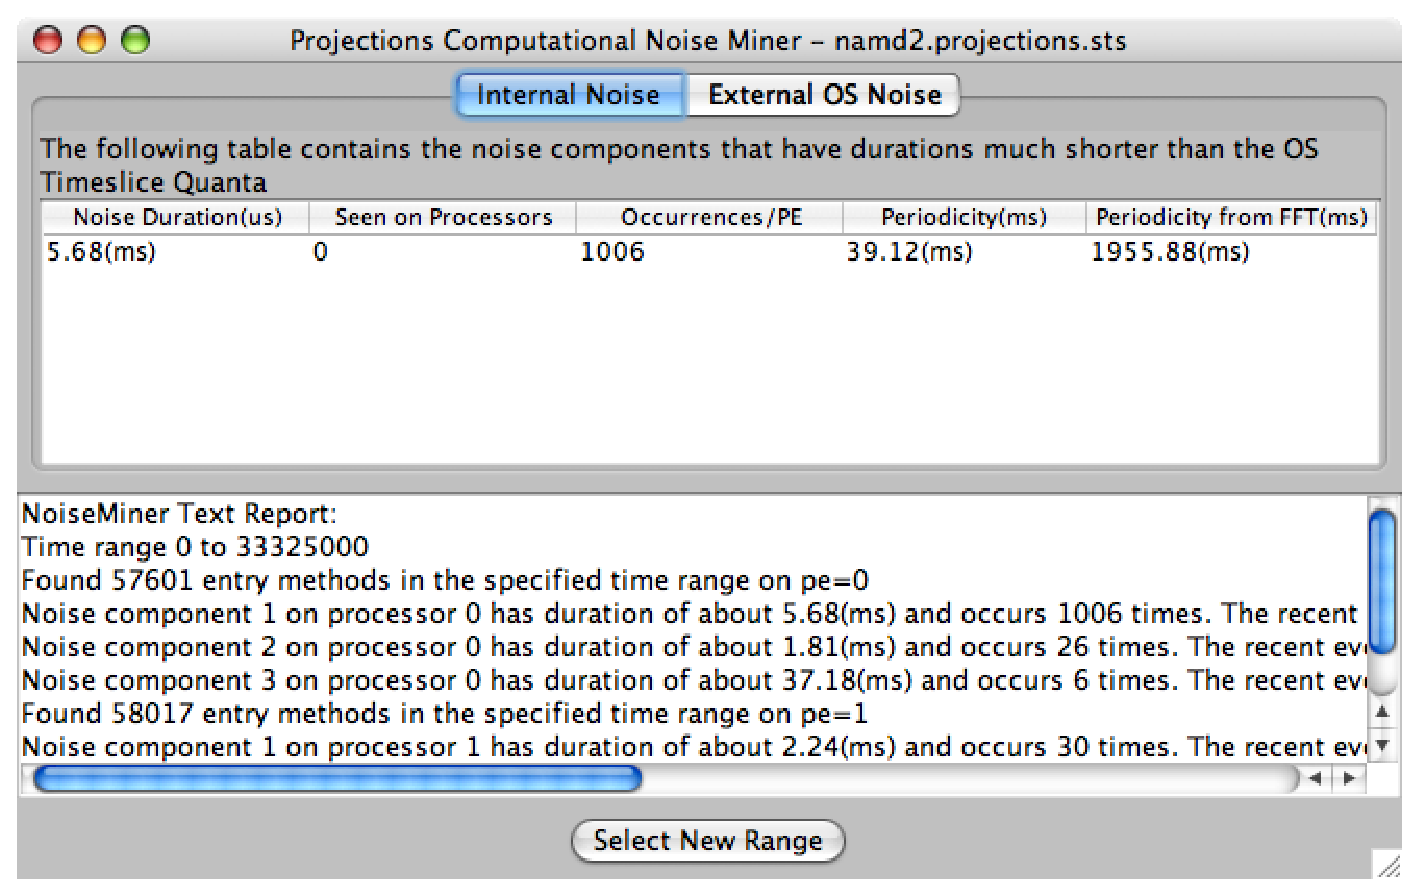
\includegraphics[width=4.0in]{fig/noiseminer}
\caption{NoiseMiner View}
\label{noiseminer}
\end{figure}

NoiseMiner works by storing histograms of each entry method's duration. The histogram bins contain a window of recent occurrences as well as an average duration and count. After data stream has been parsed into the histogram bins, the histogram bins are clustered to determine the ``normal'' entry method duration. The histograms are then normalized by the ``normal'' duration so that they represent the abnormally stretched amounts for the entry methods. Then the histogram bins are clustered by duration and across processors. Any clusters that do not contribute much to the overall runtime are dropped. Finally each cluster is reported as shown in figure \ref{noiseminer}. The resulting clusters are displayed in one of two tabs: the \textit{Internal Noise} tab will list any events width periodicity significantly shorter than the OS time quantum which is currently hard-coded to 100ms while the \textit{External Noise} tab will list any events width periodicity close to or longer than the OS time quanta. A slightly more detailed text report is also provided in the bottom pane of the window for user's wishing to record the information for future reference.